\documentclass[tikz,border=10pt]{standalone}
\usetikzlibrary{shapes.geometric, arrows.meta}

\tikzset{
    block/.style = {rectangle, draw, fill=blue!20, 
        text width=6em, text centered, rounded corners, minimum height=3em},
    line/.style = {draw, -Stealth, thick}
}

\begin{document}

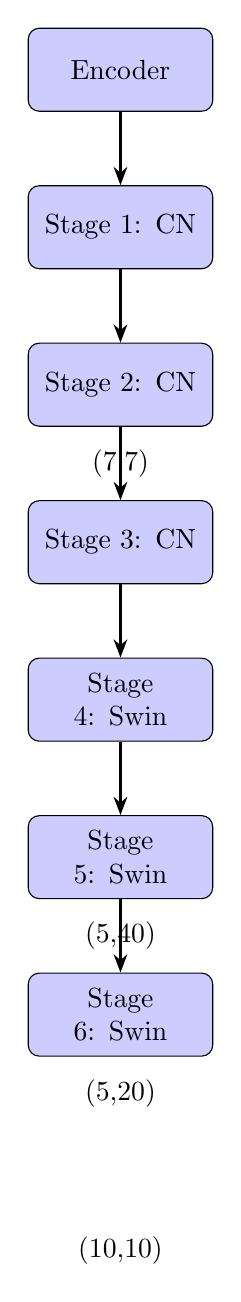
\begin{tikzpicture}[node distance=2cm]

\node [block] (encoder) {Encoder};
\node [block, below of=encoder] (stage1) {Stage 1: CN};
\node [block, below of=stage1] (stage2) {Stage 2: CN};
\node [block, below of=stage2] (stage3) {Stage 3: CN};
\node [block, below of=stage3] (stage4) {Stage 4: Swin};
\node [block, below of=stage4] (stage5) {Stage 5: Swin};
\node [block, below of=stage5] (stage6) {Stage 6: Swin};

% Connections between stages
\draw [line] (encoder) -- (stage1);
\draw [line] (stage1) -- (stage2);
\draw [line] (stage2) -- (stage3);
\draw [line] (stage3) -- (stage4);
\draw [line] (stage4) -- (stage5);
\draw [line] (stage5) -- (stage6);

% Adding dimensions and parameters
\node [below of=stage1, yshift=-1cm] (cn_params) {(7,7)};
\node [below of=stage4, yshift=-1cm] (swin_params_1) {(5,40)};
\node [below of=stage5, yshift=-1cm] (swin_params_2) {(5,20)};
\node [below of=stage6, yshift=-1cm] (swin_params_3) {(10,10)};

\end{tikzpicture}

\end{document}